\documentclass[]{report}
%[dvips]
\usepackage{graphicx}
\usepackage{tabularx}
\usepackage{subfigure}
\usepackage{afterpage}
\usepackage{amsmath,amssymb}            
\usepackage{rotating}  
\usepackage{fancyhdr}  
\usepackage[scriptsize]{caption} 
\hyphenation{a-gen-tiz-za-zio-ne}


%\addtolength{\oddsidemargin}{-0.5 cm}
%\addtolength{\evensidemargin}{-0.8 cm}
%\addtolength{\textwidth}{2.3 cm}
%\addtolength{\topmargin}{-2.20 cm}
%\addtolength{\textheight}{4.45 cm}
\linespread{1.1}

\usepackage[english]{babel}
\usepackage[latin1]{inputenc}
\renewcommand{\captionfont}{\normalfont \sffamily \itshape \small}

\pagestyle{fancy}

\begin{document}

\pagenumbering{Roman}
\renewcommand{\headrulewidth}{0 pt} 
\documentclass[]{book}

\usepackage{graphicx}

\begin{document}

\thispagestyle{empty}
%\begin{titlepage}
\vspace*{-1.5cm} \bfseries{
\begin{center}
	
	\large
  		POLITECNICO DI MILANO\\
  	
  	\normalsize
  		Corso di Laurea \textbf{MAGISTRALE} in Ingegneria Informatica\\
  		Dipartimento di Elettronica e Informazione\\
  		
  	\begin{figure}[htbp]
   		\begin{center}
      		
\includegraphics [width = 3.5 cm]{./pictures/logopm}
    	\end{center}
  	\end{figure}
  	
\end{center}

\vspace*{2 cm}
\begin{center}
  	
  	\vspace*{0.3 cm} \LARGE

	\textbf{}\\

	\vspace*{.75 true cm} \large
  
  		NECST Lab \\
  		Novel, Emerging Computing System Technologies Laboratory\\
  		
\end{center}

\vspace*{3.0 cm} \large

\begin{minipage}[b]{.45\linewidth}
	\begin{flushleft}
  		Relatore: \\
  		Correlatore: \\ 
	\end{flushleft}
\end{minipage}
\begin{minipage}[b]{.45\linewidth}
	\begin{flushright}
  		Tesi di Laurea di:\\ 
	\end{flushright}
\end{minipage}

\vspace*{0.5 cm}

\begin{center}
	Academic Year 2015-2016
\end{center} \clearpage

}

\end{document}

\normalfont \cleardoublepage
\vspace{17cm}
\thispagestyle{empty}
%\large
\begin{flushright}
\itshape{ To someone...}
\end{flushright}


\cleardoublepage
\newpage
\chapter*{Summary}

\addcontentsline{toc}{chapter}{Summary}

\chapter*{Thanks}

\addcontentsline{toc}{chapter}{Thanks}


\pagenumbering{arabic}
\normalfont
\renewcommand{\chaptermark}[1]{\markboth{\thechapter.\ #1}{}} 
\renewcommand{\sectionmark}[1]{\markright{\thesection.\ #1}}         
%\fancyhead[LE,RO]{\bfseries\thepage}    
\fancyhead[RE]{\bfseries\leftmark}    
\fancyhead[LO]{\bfseries\rightmark}     
\renewcommand{\headrulewidth}{0.3 pt} 
\chapter{Introduction}
\label{Introduction}
\thispagestyle{empty}



\chapter{Motivation}
\label{chapter2}
\thispagestyle{empty}

\section{Packed malware problem}
\paragraph{}
In order to avoid \ac{AV} detection and harden the process of reverse engineering usually malware hide and protect their code employing different techniques and tools. This process, generally called \textit{packing}, makes the static analysis of a binary almost completely useless.\\
There are lots of different run-time tools available in order to compress, encrypt, protect both good and malicious software, the main categories in which this tools fall are:
\begin{itemize}
\item \emph{Packer}: a packer usually tries to reduce the size of a binary by using different compression algorithms.
\item \emph{Crypter}: the goal of a crypter is to encrypt the executable and hardening the disassembly.
\item \emph{Protector}: a protector implements different anti-debugging and generally anti-reversing techniques in order to protect the binary's copyright in the case of a good program, or hide the malicious code in case of a malware.
\item \emph{Virtualizer}: a virtualizer translates the code of the original program into a new  instruction set and  interprets it at runtime.
\end{itemize}
All these tools change deeply the original \ac{PE} file by modifying the \ac{OEP}, the \textit{Import directory} table and many other resources and fields. Usually they are mixed together in order to obtain a more advanced protection tool that in this work we will refer generally as \textit{packer}.\\
A \textit{packer} is the tool that implements the previously described functions: it receives in input a \ac{PE} file that represent a Windows program, transforms and obfuscates its code/resources and then appends new codes, called \textit{stub}, that will \textit{unpack} the original one runtime once the program is executed.
\begin{figure}[!ht]
	\begin{center}
   		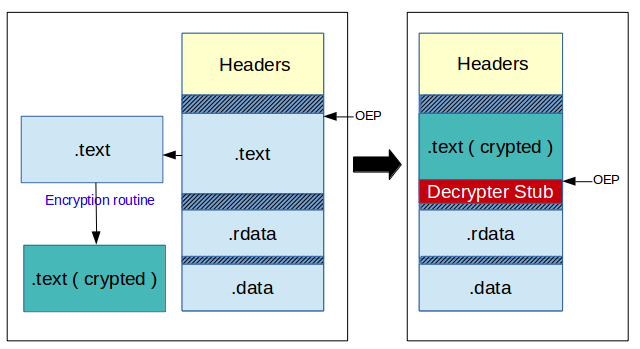
\includegraphics[width=\textwidth]{pictures/packer_general.png}
	\end{center}
	\caption{A general packer}
\end{figure}
Malware writers can decide to use an \textit{off-the-shelf} packer (commercial or free) or to implement their own solution with a \textit{custom packer}. The complexity of \textit{packers} can be very different: from those which write and execute directly the original code, to others that employ multiple unpacking routines and obfuscation techniques such as runtime repacking of previously unpacked code.\\
This process has different consequences both in the \ac{AV} detection and manual analysis of malicious binary:
\begin{itemize}
\item Usually \acp{AV} employ different static analysis techniques in order to understand if a file is malicious or not, but packing a binary destroys any possibility to understand what the program will do on the system without executing it, and so voids any effort from the point of view of a static analysis.
\item The process of reverse engineering a packed malware can be very time consuming and since lots of malware is pushed every day on the internet there is the necessity of fast analysis and fast updating of \ac{AV} software.
\end{itemize}
\paragraph{}
These problems inspired different works in building an automatic generic unpacker aimed to extract the original code from the packed one. Some of them are more oriented in detection of malicious packed program helping an \ac{AV} software on end users PCs, others are instead proposed as tools for speed up the work of professional malware analysts.
\paragraph{}
A comprehensive study and a taxonomy of the levels of complexity of nowadays packers have been presented by Ugarte-Pedrero et al\cite{sokpacker}. 
In order to clarify better what a packer is and how it operates we will discuss in the next chapter the main points of the previously mentioned research.

\subsection{Packer taxonomy}
\paragraph{}
As previously explained a packer can implement different obfuscation techniques in order to harden the analysis of a program. In this chapter we are going to analyse the proposed taxonomy in order to better understand the goals of our work and its limitation against the current packing methods.\\
Before starting to present the techniques we need to define some terms that are essential in order to understand how a packer works: 
\begin{itemize}
\item \textit{Layer}: a layer is a set of contiguous memory addresses that are executed after being written. A layer can unpack another unpacking-layer or layer that contains the original program code
\item \textit{Transition}: a transition is a control transfer from a layer to another layer: it can be a \textit{forward transition} if the execution goes from a previously unpacked layer to a newer layer, or a \textit{backward transition} if the execution goes from a newer layer to an older one. From this definition we can derive the concept of \textit{linear unpacking}, in which all the transition are \textit{forward transitions}, and \textit{cyclic unpacking}, in which there are some \textit{forward transitions} and some \textit{backward transitions}
\item \textit{Tailed/Interleaved}: we say that a packer is tailed if there is soon or later a transition from the unpacking layers to the original program code and then the execution never returns to the unpacking layers. Contrary we say that the unpacking is \textit{interleaved} if the execution bounces between the unpacking layers and the original program code
\item \textit{Frame}: a frame is a portion of original program code unpacked and executed. A \textit{mono frame} packer means that the unpacking routine will reveal all the original code before jumping and executing it; contrary a \textit{multi frame} packer unpacks only a slice of the original program code, executes it and then unpacks another slice of original program code and so on. A \textit{multi frame} behavior can be \textit{incremental} if the slices of original program are revelead in order following the original program execution and never re-encrypted again, contrary a \textit{shifted frames} policy reveal only one slices at times and re-encrypt the slice once executed
\end{itemize}
\paragraph{}
As proposed by Ugarte-Pedrero et al\cite{sokpacker} we are going to identify the complexity of a packer by using a scale from 1 to 6.

\subsubsection{Type 1 packer}
The simplest form of packers are \textit{single layer} packers: they runtime unpack the original binary using a single stub and then jump to it with a \textit{tail jump}. 
\begin{figure}[!ht]
	\begin{center}
   		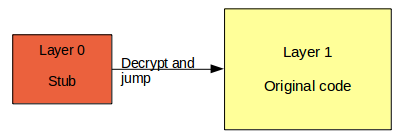
\includegraphics[width=0.7\textwidth]{pictures/packer_type_1.png} 
	\end{center}
	\caption{Type 1 packer}
\end{figure}
This scheme is typical of packers like UPX, EXEpacker.

\subsubsection{Type 2 packer}
The packers in this category are defined as \textit{multi-layer} and \textit{linear}. This means that they employ different layers and the transitions between them are always from the older to the newer. Also this kind of packers are defined as \textit{tailed} since the last jump redirects the execution at the original program code.\\
\begin{figure}[!ht]
	\begin{center}
   		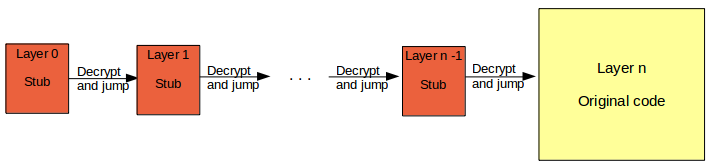
\includegraphics[width=\textwidth]{pictures/packer_type_2.png}
	\end{center}
	\caption{Type 2 packer}
	\label{Type 2 packer}
\end{figure}
We can see from Figure \ref{Type 2 packer} that the layer 0 unpacks and jumps to the layer 1, then the scheme is repeated until the layer (n-1), which decrypts and finally jumps to the original code. All the layers from 0 to n-1 are part of the packer stub.

\subsubsection{Type 3 packer}
These packers are defined as \textit{multi-layer}, \textit{cyclic} and \textit{tailed}. This means that they employ different layers and the transitions are both \textit{forward transition} and \textit{backward transition}.\\
\begin{figure}[!ht]
	\begin{center}
   		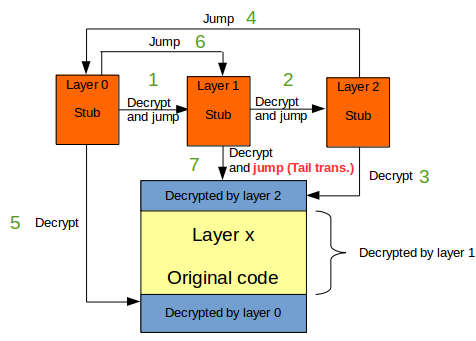
\includegraphics[width=0.9\textwidth]{pictures/packer_type_3.png} 
	\end{center}
	\caption{Type 3 packer}
	\label{Type 3 packer}
\end{figure}
Following the numbers reported in Figure \ref{Type 3 packer} let's explain briefly how the process of the packer's stub works in this example. Keep in mind that the scheme can change but the properties for this kind of packers remains the ones described previously.
\begin{itemize}
\item (1) The first layer decrypts and finally jumps to the layer 1
\item (2) The layer 1 does the same thing, unpacking and jumping to the layer 2
\item (3) Then the layer 2 decrypts a piece of original program code, and then (4) re-jumps with a backward transition to the layer 0
\item (5) Now the layer 0 decrypts another piece of the original program code and then (6) re-jumps to layer 1
\item (7) Finally layer 1 decrypts the last piece (Layer X) of original code and jumps to the \ac{OEP} of the program
\end{itemize}
A scheme of this type is implemented by PE-Compact, Aspack, FSG, ASprotect, NSPack, WinUpack, UPolyX and Obsidium.

\subsubsection{Type 4 packer}
These packers are \textit{multi-layer}, \textit{cyclic} and \textit{interleaved}. This means that they use different layers with both \textit{forward and backward transitions}, and during the execution of the original program the control is redirected in some way to the packer code.
\begin{figure}[!ht]
	\begin{center}
   		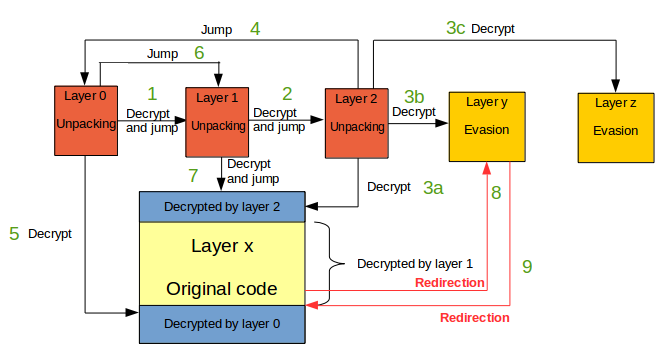
\includegraphics[width=\textwidth]{pictures/packer_type_4.png} 
	\end{center}
	\caption{Type 4 packer}
\end{figure}
\begin{itemize}
\item (1) The first layer decrypts and finally jumps to the layer 1
\item (2) The layer 1 does the same thing, unpacking and jumping to the layer 2
\item (3a) The layer 2 decrypts a piece of original code and (3b+3c) two additional layers that will implement, for example, some evasion techniques like debugger detection. After this (4) it jumps with a backward transition to layer 0
\item (5) Now layer 0 decrypts another piece of original program and then (6) jumps to layer 1 again
\item (7) Layer 1 finally decrypts and jumps to the original program \ac{OEP}
\item (8) During program execution the packer re-gains control executing the evasion routines; this is usually implemented by hijacking the \ac{API} called by original program
\item (9) After the evasion code has been executed the execution can resume to the original program code or into other location based on the results of the evasion checks implemented
\end{itemize}
A scheme of this type is implemented by ACProtect.

\subsubsection{Type 5 packer}
Packers of this type are \textit{multi-layer}, \textit{cyclic}, \textit{interleaved} and \textit{multi frame} with an \textit{incremental frames} behaviour. This means that they use different layers with both \textit{forward and backward transitions}, during the execution of the original program the control is redirected in some way to the packer code and the original program code is revealed slice by slice when needed to execute. Like the previous packer's type also here exists a moment in which all the original program code is unpacked in memory, but differently in this case dumping at the \ac{OEP} does not permit to dump all the original program code, since it is still encrypted in memory; nonetheless, a theoretical dump nearly the end of execution can dump the entire program's code.
\begin{figure}[!ht]
	\begin{center}
   		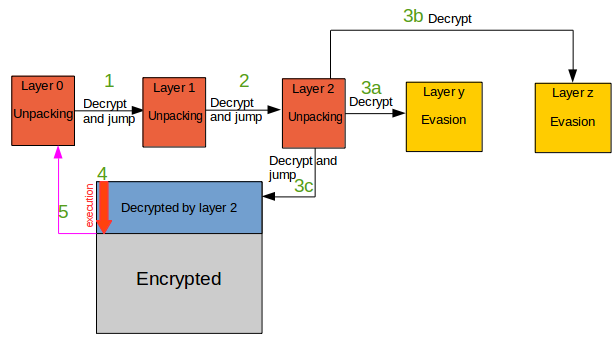
\includegraphics[width=\textwidth]{pictures/packer_type_5-1.png}
	\end{center}
	\caption{Type 5 packer (I)}
\end{figure}
\begin{itemize}
\item (1) The layer 0 unpacks and jumps to layer 1
\item (2) The layer 1 unpacks and jumps to layer 2
\item (3a+3b) Layer 2 unpacks two additional layers that will implement some kind of evasion techniques. Finally (3c) it unpacks a slice of original program's code at the \ac{OEP} and redirects the execution there, (4) starting to execute the original program
\item (5) The execution reaches the end of the unpacked original program's code and supposedly an exception will be launched. The packer catches this exception and redirects the execution to layer 0
\end{itemize}
\begin{figure}[!ht]
	\begin{center}
   		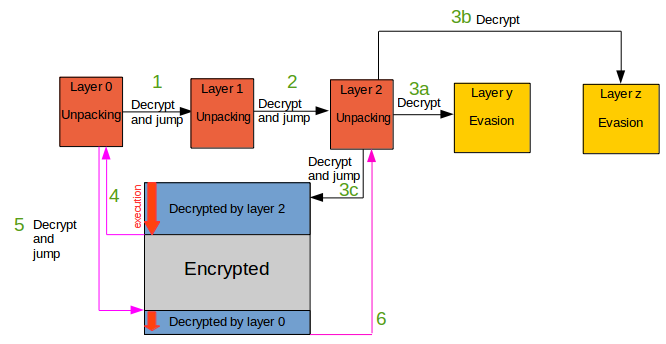
\includegraphics[width=\textwidth]{pictures/packer_type_5-2.png}
	\end{center}
	\caption{Type 5 packer (II)}
\end{figure}
\begin{itemize}
\item (5) Layer 0 decrypts on demand a new slice of original program's code and then jumps to it
\item (6) The same things as before happen when execution reaches again the end of the previously unpacked code, and now the layer 2 take control
\item (7) Layer 2 decrypts the last slice of original program's code and finally jumps to it. As before in (8) there is a redirection to an evasion layer that can decide to (9) resume the execution to the original program's code or to abort the execution depending on its checks.
\end{itemize}
\begin{figure}[!ht]
	\begin{center}
   		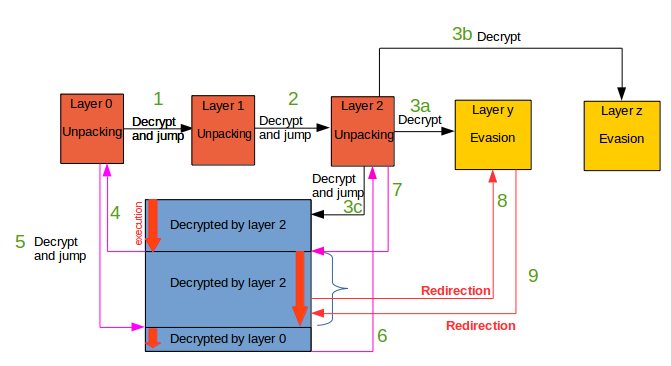
\includegraphics[width=\textwidth]{pictures/packer_type_5-3.png}
	\end{center}
	\caption{Type 5 packer (III)}
\end{figure}

\subsubsection{Type 6 packer}

Packers of this type are \textit{multi-layer}, \textit{cyclic}, \textit{interleaved} and \textit{multi frame} with a \textit{shifted frames} behaviour. This means that they use different layers with both \textit{forward} and \textit{backward transitions}, during the execution of the original program the control is redirected in some way to the packer's code and the original program code is revealed slice by slice and re-encrypted once executed; packers with such complexity never let all the program code to live in memory, so a dump that encompass the entire original program's code does not exists.
\begin{figure}[!ht]
	\begin{center}
		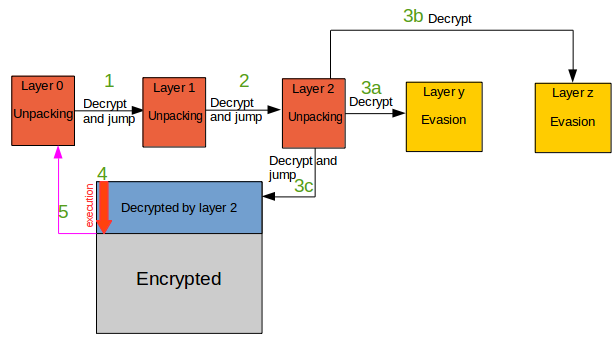
\includegraphics[width=\textwidth]{pictures/packer_type_5-1.png}
	\end{center}
	\caption{Type 6 packer (I)}
\end{figure}
\begin{itemize}
\item (1) The layer 0 unpacks and jumps to layer 1
\item (2) The layer 1 unpacks and jumps to layer 2
\item (3a+3b) Layer 2 unpacks two additional layers that will implements some kind of evasion techniques. Finally (3c) it unpacks a slice of original program's code at the \ac{OEP} and redirects the execution there, (4) starting to execute the original program
\item (5) The execution reaches the end of the unpacked original program's code and supposedly an exception will be launched. The packer catches this exception and redirects the execution to layer 0
\end{itemize}
\begin{figure}[!ht]
	\begin{center}
		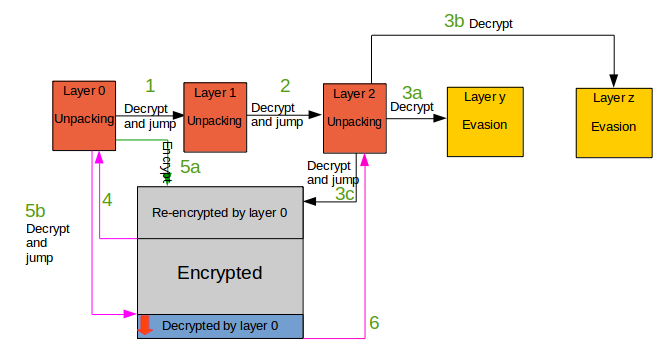
\includegraphics[width=\textwidth]{pictures/packer_type_6-1.png}
	\end{center}
	\caption{Type 6 packer (II)}
\end{figure}
\begin{itemize}
\item (5a) Layer 0 re-encrypts the previous slice of original program's code, and (5b) decrypts on demand a new slice of original program's code; finally it jumps to the new unpacked slice
\item (6) The same things as before happen when execution reaches again the end of the previously unpacked code, and now the layer 2 takes control
\end{itemize}
\begin{figure}[!ht]
	\begin{center}
		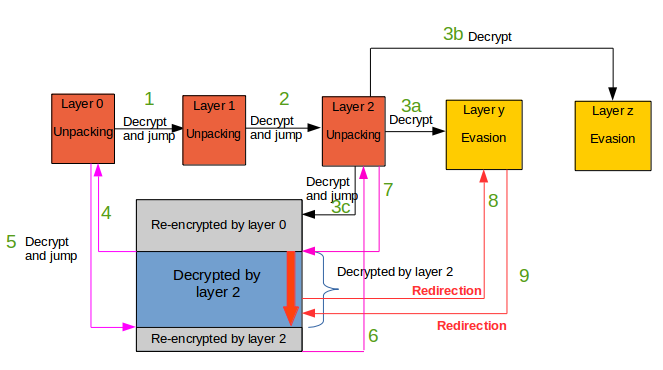
\includegraphics[width=\textwidth]{pictures/packer_type_6-2.png}
	\end{center}
	\caption{Type 6 packer (III)}
\end{figure}
\begin{itemize}
\item (7) Layer 2 re-encrypts the previous slice of original program's code and decrypts the last slice, jumping to it at the end. As before, in (8) there is a redirection to an evasion layer that can decide to (9) resume the execution to the original program's code or to abort the execution depending on its checks
\end{itemize}
A scheme of this type is implemented by Armadillo.

\subsubsection{Packer complexity distribution}
\paragraph{}
According to Ugarte-Pedrero et al\cite{sokpacker}, the distribution of packer complexity resulted from the analysis of 6088 packed malware binaries is the following:

\begin{table}[H]
\begin{center}
\begin{tabular}{l*{6}{c}r}
Type      & Off-the-shelf & Custom packers \\
\hline
Type 1 &       173 (25.3\%) & 443 (7.3\%) \\
Type 2 &       56 (8.2\%) & 752 (12.4\%) \\
Type 3 &       352 (51.4\%)  & 3993 (65.6\%) \\
Type 4 &       86 (12.6\%) & 843 (13.8\%) \\
Type 5 &       6 (0.9\%)  & 46 (0.8\%) \\
Type 6 &       12 (1.8\%) & 11 (0.2\%) \\
\end{tabular}
\end{center}
\end{table}

Interpreting the data we can derive that:
\begin{itemize}
\item Malware writers seems to prefer using a custom packer rather than relying on an existing ones
\item more than 90\% of the binary packed with both an off-the-shelf/custom packer use a complexity that ranges from 1 to a maximum of 4. This suggests that a generic unpacker that can handle such complexities can cover a good number of cases
\item In both cases of an off-the-shelf/custom packer we can see that the preferred complexity seems to be a Type 3 packer. This could be an indication that a complexity of that level is enough to defeat the nowadays \ac{AV} solutions
\item The use of a complexity greater than Type 4 is rarely used
\end{itemize}
As presented, the complexity of a packer can escalate really quickly and building a generic unpacker that can cover all these schemes is a big challenge.

\section{State of art}
\paragraph{}
Lots of different tools using different approaches and techniques have been proposed. 
The approaches for automatic unpacking can be very different:
\begin{itemize}
\item \textit{Static unpacking}: this can sound counterintuitive, but some works proposed to identify unpacking routines inside the binary and reconstruct an ad hoc unpacker for the binary starting from these routines. This approach has got numerous limitation but can lead to interesting result in some case as demonstrated by Coogan et al.\cite{coogan}
\item \textit{Hybrid unpacking}: this mixes some static heuristics with dynamic analysis.
\item \textit{Dynamic unpacking}: these techniques follow the idea to let the unpacker do its work and then try to extract runtime the unpacked code. 
\end{itemize}
\paragraph{}
Depending on the purpose of the tool there are different requirements that a generic unpacker must respect. If the aim is to help the AV on end users' PCs:
\begin{itemize}
\item Safety: try to recognize the malicious behaviour as fast as possible and block the execution. 
\item Performance: it should not slow down too much the execution of AV scans.
\end{itemize}
Note that in these cases, the scope is not to reconstruct a binary from a packed one, but rather to stop malicious behaviours when they manifest. \\
In this area have been done works such as OmniUnpack and JustIn.
\paragraph{}
On the other side if the aim is to help the analysis in a laboratory:
\begin{itemize}
\item Fidelity: the unpacked binary extracted by the tool should be equal to the one that would be unpacked normally. 
\item Generality: the unpacker can not be focused only against one packer but should unpack different of them with one generic algorithm.
\end{itemize}
In this case we do not care so much about safety because usually analysis is performed inside a controlled environment and the analysts want to observe the complete execution of malware. Also the performances are not a critical feature here because we are not constrained by user experience needs.\\
In this category have been developed tools like PolyUnpack, Ether, Eureka, Renovo, Lynx.
These tools merely collect dumps of the binary while unpacking and they don't reconstruct a fully runnable binary given a packed one.


\section{Challenges}
\subsection{Determine the Original Entry Point of the malware}

\subsection{Reconstruct the Import Table despite IAT obfuscation}

\paragraph{}
Since our work is a component of a bigger malware analysis platform\cite{jackdaw}, our tool is oriented to help malware analyst during the reversing process of a packed binary. 
Our approach aims not only to unpack the malware, but also to reconstruct a fully working unpacked binary. To do so, we not only have to identify the original entry point (OEP) and dump the code at that moment, but we have to find the IAT inside the process and reconstruct a correct import directory in the final PE file.\\
According to the discussion about packer's complexity our aim is to unpack untill Type 4 since, as presented by Ugarte-Pedrero et al\cite{sokpacker} in their packer's complexity distribution, more than 90\% of the binary packed with both an off-the-shelf/custom packer use a complexity that range from 1 to a maximum of 4.
\paragraph{}
The first thing we have to deal with are the unpacking routines of the packers: every time the execution of the malware comes from a previously written memory area, then it could be a sign that the unpacking stage has finished or that a new unpacking layer has started.\\
We have also to deal with techniques of IAT obfuscation: some malwares can do this in order to make difficult to statically analyse them to understand what they are doing.

\section{Goals}
\subsection{Develop a generic automatic unpacker}
\subsection{Obtain a reconstructed and working PE}
\chapter{Approach}
\label{chapter3}
\thispagestyle{empty}

\section{Dynamic Binary Instrumentation}
\paragraph{}
Dynamic Binary Instrumentation is a technique for analysing the behaviour of a binary application through the injection of instrumentation code. The instrumentation code can be developed in an high level programming language and is executed in the context of the analysed binary with a granularity up to the single assembly instruction. The injection of instrumentation code is achieved by implementing a set of callbacks provided by the DBI framework. The most common and useful callbacks are:
\begin{itemize}
 \item Instruction callback: invoked for each instruction
 \item Image load callback: invoked each time an image (dll or Main image) is loaded into memory
 \item Thread start callback: invoked each time a thread is started
\end{itemize}
Besides the callbacks the DBI framework allows to intercept and modify operative system APIs and system calls and this is very useful to track some behaviours of the binary, like the allocation of dynamic memory areas.


\section{Approach overview}
\paragraph{}
Our tool exploits the functionalities provided by the Intel PIN Dynamic Binary Instrumentation frameworks to track the memory addresses which are written and then executed with an instruction level granularity.
More in details for each instruction the following steps are performed:
\begin{enumerate}
\item Instruction Filtering: ignore the effects of a particular set of instructions for performance reasons;
\item Written addresses tracking: keep track of each memory address which is written in order to create a list of memory ranges of contiguous writes defined \textit{Write Intervals} .
\item \textit{Write xor execution} instructions tracking: check if the currently executed instruction belongs to a \textit{Write Interval}. This is a typical behaviour in a packer that is executing the unpacked layer and for this reason we trigger a detailed analysis which consists of:
	\begin{enumerate}
	\item Dumping the main image of the PE and a memory range on the heap depending on the address of the current instruction;
	\item Reconstructing the IAT and generating the correct Import Directory;
	\item Applying some heuristics to evaluate if the current instruction is the OEP;
	\end{enumerate}
\end{enumerate}
The result of our tool is a set of memory dumps or reconstructed PE depending on the result of the IAT fixing phase and a report which includes the values of each heuristics for every dump. Based on these information we can choose the best dump, that is the one that has the greatest chance of work.\\

\section{Approach details}
\paragraph{}
In this section we are going to describe in details the steps introduced in the previous section.
\paragraph{}
During the development we have adapted our approach in order to increase speed and effectiveness of our tool. Following there is a detailed explanation of our improvements on the initial approach:
\begin{enumerate}
\item in the first step, we add the option of not to track writes of library instructions on the stack and in the TEB
\item in the second step we filter instructions of known libraries before dumping
	\begin{enumerate}
	\item when trying to reconstruct the IAT we added some code in order to deal with 			obfuscation techniques like \textit{IAT Redirection} and \textit{Stolen API}
	\item we implemented five heuristics:
		\begin{itemize}
		\item entropy: check if the value of the entropy is above a certain threshold
		\item long jump: check if the "distance" between the current EIP and the previous 			one is above a certain threshold
		\item jump outer section: check if the current EIP is a different section from the 		one of the previous EIP
		\item pushad popad: check is a pushad popad has been found in the trace
		\item init function calls: check if the imports of the dump are function commonly 			 used by the malware and not by the unpacking layers
		\end{itemize}
	\end{enumerate}
\end{enumerate} 
For the instructions that execute from the same write set we adopted the following approach: if the "distance" between the current EIP and the EIP of the previous instruction is above a given threshold then we do the same as if we were in the case 2, otherwise we jump to the next instruction.\\
Finally, we are noticed that dumping only the main executable in memory is not enough because some packers dump the final payload on the heap. In order to deal with it, we track heap allocations and writes inside an heap interval. If necessary, we dump these intervals too.

\subsection{Instructions Filtering}
\paragraph{}
Since our tool works with an instruction level granularity, limiting our analysis to the relevant instruction of the program is a critical point. For this reason we have introduced some filters, based on the common behaviours showed by the packers, which make our tool ignore the effects of a set of instructions. More in detail two kind of instructions are not tracked by default:
\begin{itemize}
	\item Write instruction on the TEB and on the Stack
	\item Instruction executed by known Windows Libraries
\end{itemize}
The write instructions on the stack are ignored because unpacking code on the stack is not common compared to unpacking it on the heap or inside the main image. Moreover many instructions write on the stack and keeping track of all the written addresses would downgrade the performances gaining little advantages against a very small set of packers.\\
The same considerations can be applied to the instructions which write on the TEB, since most of these writes are related to the creation of instruction handlers and there is very little chance that a packer uses this addresses to unpack the encrypted payload.\\
The instructions executed by known Windows Libraries are never considered when checking if the current instruction address is contained inside a \textit{Write Set} because this would mean that the packer writes the malicious payload in the address space of a know Windows Library. This behaviour has never been identified in the packer analysed; moreover, this could introduce some crashes if the application explicitly use one of the functions which have been overwritten.

\subsection{Heuristics description}
\paragraph{}
Our tool makes a dump each time the WxorX law is broken in a new \textit{Write Set} or in an existing one if \textit{InterWriteSet} analysis is enabled. Consequently, at the end of the execution we may have a lot of dumps and check them manually can be very time-consuming. Heuristics help in automatically identify the dumps that are most likely to work and also provide a "best dump", the one with the greatest chance to be the contain the original unpacked code.\\ 
As described in \cite{Practical_Malware_Analysis}, entropy can be considered as a measure of the disorder of a program. For example, random data have the highest possible entropy. Since compressed or encrypted data more closely resembles random data, entropy can be used in detecting if an executable has been compressed, encrypted or both. Usually
\chapter{Implementation details}
\label{chapter4}
\thispagestyle{empty}

\section{System architecture}

\section{System details}
\paragraph{}
In this section we are going to focus in detail about the implementation of each of the six points listed in the previous chapter:
\begin{enumerate}

\item The techniques used in order to retrieve the real EIP exploit some assembly instructions which need to save the execution context, including the instruction pointer value, in order to work correctly. Some of these are the instructions that trigger exceptions (E.g. INT 2E) or those that save the floating point unit state (E.g. FSAVE). In order to deal with these techniques we perform a single instruction analysis, and if we find one of these instructions, after its execution, we restore the context with a fake EIP value (The one that the program would have seen if it was run without PIN).

\item A common method used to detect a Just In Time compiler is to write a small routine at the beginning of \textit{ZwAllocateVirtualMemory} (frequently used by JIT) which increments a counter every time it is called with the following two parameters : 

\begin{itemize}
\item AllocationType MEM\_COMMIT and MEM\_RESERVEs

\item Protect = PAGE\_EXECUTE\_READWRITE
\end{itemize}

If the counter becomes bigger than a threshold the pin tool has been detected. We avoid this technique analysing all the write operations made by the instrumented program, and when one of these is attempted in the protected memory range, identified as the beginning of the API \textit{ZwAllocateVirtualMemory}, it is redirected into another memory address.

\item the eXait library uses the function \textit{VirtuaQuery} to retrieve information about the page permissions. In order to avoid this we hooked the \textit{VirtuaQuery} and when the program queries pages outside the whitelist we fake the results and return that those pages are not mapped. Moreover, the \textit{VirtuaQueryEx} has the same function of the \textit{VirtuaQuery} but it allows to specify a handle of the process whose pages we want to query. However, if the handle corresponds to the current process, the \textit{VirtuaQueryEx} does exactly the same things as the \textit{VirtuaQuery}. In order to prevent this, we patched also the \textit{VirtuaQueryEx}.

\item To avoid the readings made by the instrumented process in the memory region in which reside dlls, code patterns or resources necessary to the DBI, we have built a whitelist with all the memory area in which a process is allowed to read (stack, sections, the runtime dynamic allocated memory, mapped file). If the process tries to access resources outside those in the whitelist, we return random data to avoid leak of PIN artefacts.

\item A process can retrieve the time from the system in three main different ways and we developed three techniques in order to lower correctly the time value returned :

\begin{itemize}
\item Detect the reads on the KUSER\_SHARED\_DATA structure, where tick count and clock cycles passed are stored, and divide it by a configurable divisor.

\item Hook the system call \textit{NtQueryPerformanceCounter} and fake, in the same way as the point above, the returned result using a different divisor.

\item Intercepted the \textit{rtdsc} assembly instruction and fake the value returned in the registers EAX and EDX.
\end{itemize}

\item Based on a survey \cite{Controlling-Windows-process-list} of the most frequent techniques employed to discover the parent process we implemented some countermeasures in order to fake the list of processes:

\begin{itemize}
\item Hook the system call \textit{NtQueryProcessInformationSystem} in order to modify the returned process list changing the name \textit{pin.exe} in \textit{cmd.exe}

\item Hook the system call \textit{NtOpenProcess} and, if the process that has to be open is \textit{csrss.exe} return the status of the operation as NTSTATUS\_ACCESS\_DENIED
\end{itemize}

\end{enumerate}


\chapter{Experimental validation}
\label{chapter5}
\thispagestyle{empty}

\section{Goals}
With our experiments we want to show the effectiveness of our tool. During the development we did some preliminary tests on normal programs: we packed them with common packers and tried our tool on them. Then results were pretty convincing, our tool correctly unpack sample programs packed with the following packers:
\begin{itemize}
\item UPX
\item FSG
\item Yoda Crypter
\item mew
\item mpress
\item PECompact
\item ASProtect
\end{itemize}
Moreover, we are able to dump the program at the entry point, but not to reconstruct the IAT, for executables packed with:
\begin{itemize}
\item Themida, but a version without the anti-evasion flag activated
\item Obsidium, but a version without the anti-debugging flag activated
\end{itemize}
We are able to produce not working dumps also for executables packed with ASPack.

\section{Dataset}
We built our dataset from the database of VirusTotal. Using a python script we were able to write a specific query to download only packed executables. We put these malwares in a shared folder between the host and the guest system.

\section{Experimental setup}
In order to automatize we created a .bat script on the host machine that is able to restore, start, wait for 10 minutes and close the VirtualMachine using VBoxManage, the command line tool for VirtualBox.\\
At the start up of the Virtual Machine, a python script is set to automatically move a malware sample from the shared folder into the Virtual Machine and then trigger the execution of PIN with all the command line arguments to properly analyse the sample. After 5 minutes, it eventually stops the execution of PIN.\\
The final results are then moved into the shared folder with the host, in order to not lose them at the restoring of the Virtual Machine.\\
In conclusion, our system goes through the following steps:
\begin{enumerate}
\item download samples from VirusTotal and put them in the shared folder between the host and the guest machines
\item run the .bat script from the host machine which manage the Virtual Machine
\item the .bat script restores the Virtual Machine to a clean state and starts it
\item the start of the Virtual Machine triggers the execution of a python script that move the first of the samples in the guest system and starts PIN
\item after 5 minutes if PIN is still running it is stopped
\item the python script moves the results of the analysis in the shared folder
\item after 10 minutes the .bat script running in the host system stops the Virtual Machine
\item we go back to Step 3
\end{enumerate}

\section{Experiments}


\chapter{Limitations}
\label{chapter6}
\thispagestyle{empty}

\chapter{Future works}
\label{chapter7}
\thispagestyle{empty}

\chapter{Conclusions}
\label{chapter8}
\thispagestyle{empty}


\cleardoublepage
% ---- Bibliography ----
\addcontentsline{toc}{chapter}{Bibliografia}
\bibliographystyle{plain}
\bibliography{bib_thesis}
\nocite{*}

\appendix

%\pagestyle{fancy} 
\fancyfoot{}                                               
\renewcommand{\chaptermark}[1]{\markboth{\appendixname\ \thechapter.\ #1}{}} 
\renewcommand{\sectionmark}[1]{\markright{\thesection.\ #1}}         
\fancyhead[LE,RO]{\bfseries\thepage}    
                                        
\fancyhead[RE]{\bfseries\leftmark}    
\fancyhead[LO]{\bfseries\rightmark}     
\renewcommand{\headrulewidth}{0.3pt} 

\chapter{}
\label{appendix}
\thispagestyle{empty}


\end{document}





